% The entire content of this work (including the source code
% for TeX files and the generated PDF documents) by 
% Hongxiang Chen (nicknamed we.taper, or just Taper) is
% licensed under a 
% Creative Commons Attribution-NonCommercial-ShareAlike 4.0 
% International License (Link to the complete license text:
% http://creativecommons.org/licenses/by-nc-sa/4.0/).
\documentclass{article}

% My own physics package
% The following line load the package xparse with additional option to
% prevent the annoying warnings, which are caused by the package
% "physics" loaded in package "physicist-taper".
\usepackage[log-declarations=false]{xparse}
\usepackage{physicist-taper}
\makenomenclature % For an index of symbols.

\usepackage{menukeys}
\newcommand\command[1]{\texttt{\centering #1}}

\newsavebox\mybox

\newcommand\NoIndent[1]{%
  \par\vbox{\parbox[t]{\linewidth}{#1}}%
}


\title{Installation Guides}
\date{\today}
\author{Taper}


\begin{document}


\begin{lrbox}{\mybox}
\begin{lstlisting}
git clone https://github.com/VundleVim/Vundle.vim.git ~/.vim/bundle/ Vundle.vim
\end{lstlisting}
\end{lrbox}

\maketitle
\abstract{
This document installs the necessary software and plugins for
\href{https://github.com/lervag/vimtex}{Vimtex} on a Windows PC or a
Mac.  It uses a \texttt{vimrc} written by myself to free user from
configuration.  However, it does not explains the details of that
\texttt{vimrc}.
}    
\tableofcontents

\section{List of software to be installed}
\label{sec:list of software}

\begin{enumerate}
    \item \TeX Live 
        \begin{itemize}
            \item Windows: \TeX Live 2016 (\texttt{textlive2016-20160523.iso}).
            \item Mac: Mac\TeX
        \end{itemize}
    \item Vim 
        \begin{itemize}
            \item For Windows, use the latest 32bit gVim (v8.0.0540)
                \href{https://github.com/vim/vim-win32-installer/releases/}{here}
                which has \texttt{Lua} support enabled.
            \item For Mac, use the MacVim provided by Homebrew (see
                details below).
        \end{itemize}
    \item Git (v2.12.2 64bit for Windows, Mac is pre-installed with
        Git).
    \item PDF Reader that work with vimtex: SumatraPDF (v3.1.2 64bit)
        for Windows and Skim for Mac.
    \item Texstudio (v2.12.2).
    \item Python (v2.7.13 32bit). Mac comes pre-installed with Python
        2.7.
    \item A decent pure text editor:
        \begin{itemize}
            \item Windows: Notepad++ (v7.3.3), for its small size.
            \item Mac: Sublime Text
        \end{itemize}
    \item Vundle (latest commit on
        \href{https://github.com/VundleVim/Vundle.vim}{GitHub
        Vundle}), and many related plugins for Vim.
\end{enumerate}

\section{Note for Mac users}
\label{sec:Note for Mac users}

In Mac (or more generally, on any Unix OS, including Linux OS):
\begin{itemize}
    \item A \menu{\textasciitilde} means your home folder, such as \path{Macintosh HD> Users>
        YourUserName}.
    \item All files and folders starting with \menu{.} will be hidden.
        So for example, you might have trouble finding the \menu{.vim}
        folder in your \menu{\textasciitilde} folder. See this link for information
        about hidden files
        \url{http://www.macworld.co.uk/how-to/mac-software/how-show-hidden-files-library-folder-mac-3520878/}.

\end{itemize}
\section{Install Steps}
\label{sec:Install Steps}

\begin{enumerate}
    \item \TeX Live.

        \textbf{Explanation}: \TeX Live provides us with basic \TeX
        utilities and packages. Although it is big, the exhaustive
        packages it provides will be handy when we write \LaTeX{} daily.

        \textbf{For Windows}:

        First mount the ISO file (double click in Windows 8 or later,
        use third-part software in Windows 7 or earlier). Then open
        the file \texttt{install-tl-windows.bat}, and install with all
        default settings (except that you may want to change the
        installation folder).

        The installation will take a lot of time. Continue to the next
        steps while waiting for this \TeX Live installation to finish.

        \textbf{For Mac}:

        See this page: \href{https://www.tug.org/mactex/}{Mac\TeX} for
        information about it, since I don't have a Mac.

    \item (\textbf{Mac} only) Install
        \href{https://brew.sh}{Homebrew}, follow the instruction on
        that site, and you will find the life of a Mac user more
        enjoyable, especially when you are familiar with Linux.

        \textbf{Explanation}: I will install MacVim using Homebrew.

    \item Install the Vim with Lua support. 

        \textbf{Explanation}: Vim will be our editor. And \texttt{Lua}
        will provide support for some plugins of Vim.
        
        \textbf{For Windows}:

        As mentioned, \textbf{DO NOT} install the version downloaded
        from the Vim project's website. Use the link
        \href{https://github.com/vim/vim-win32-installer/releases/}{here}
        to download the version which has \texttt{Lua} support
        enabled. Install with default configuration, except that you
        will need to consider the following options:

        In this figure:
        \begin{figure}[H]
            \centering
            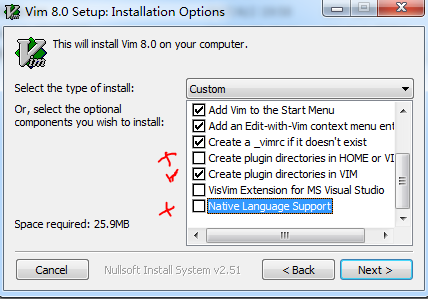
\includegraphics[width=0.6\linewidth]{pics/1.PNG}
        \end{figure}
        I encourage you
        \footnote{And if you do not follow my suggestion, you might
            need extra modification to my \texttt{vimrc} file.}
        to disable \menu{Create plugin directories in
        \texttt{HOME} or \texttt{VIM}}, and enable instead \menu{
        Create plugin directories in \texttt{VIM}}.  This make Vim put
        its plugin directory inside \texttt{VIM} folder (which is the
        folder where \texttt{VIM}) will be installed. Therefore, the Vim
        plugins would not mess up inside your \texttt{HOME} folder
        (which on Windows, people seldom touches upon), and Vim
        becomes more portable.

        I also encourage you to disable \menu{Native Language
        Support}, which force us to speak in English with Vim.

        After installation, add Vim to system \texttt{PATH} variable,
        just like what you have done when installing \texttt{Java}.

        \textbf{For Mac}: Type this into your terminal:

        \begin{verbatim} 
            brew install macvim --with-lua --with-override-system-vim
        \end{verbatim}
        
        (Now you understand how Homebrew makes your life better...
        Also, guess what those parameters do.)

    \item 
        (\textbf{Windows} only) Add Lua Support for Vim. Download
        \href{http://luabinaries.sourceforge.net/download.html}{Lua
        Binary}. The version of Lua should be consistent with the Vim
        (gVim) you installed (same OS, same architecture), and those
        DLL with MingW support are not required
        \footnote{Actually I never tested those with MingW support.
        Therefore, I do not recommand trying them.}.

        After downloading, extra the compressed file and copy the file
        \texttt{lua53.dll} \footnote{the number 53 for version may be different
        in your case. But it is the DLL file that we cared about.} and
        move it to \path{Folder Where Vim Is Installed> vim80}
        \footnote{The number $80$ is the version number of vim.} like
        this:
        \begin{figure}[H]
            \centering
            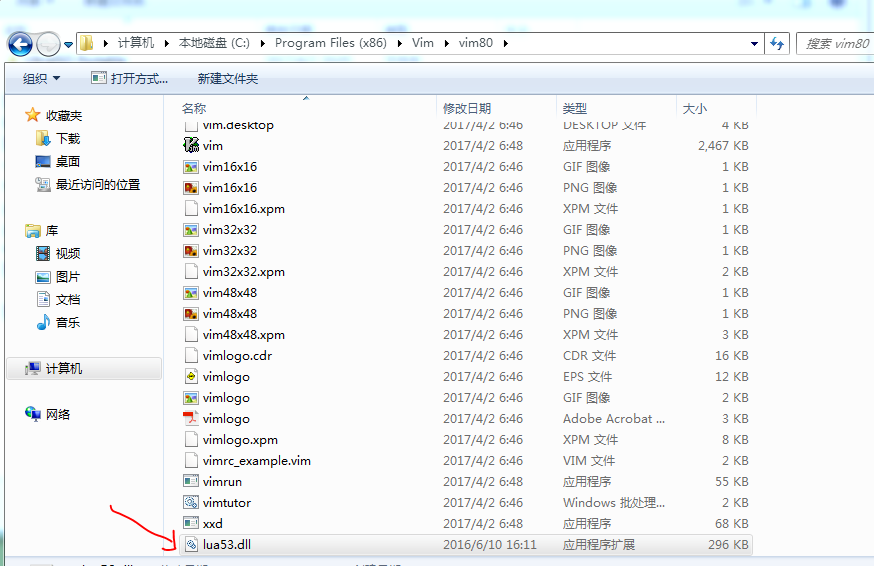
\includegraphics[width=0.6\linewidth]{pics/8.PNG}
        \end{figure}

    \item 
        (\textbf{Windows} only) Install Git, with mostly default
        option, except that you should change the default installation
        folder to somewhere you like.

        \textbf{Explanation}: Git will be used to download Vim plugins
        from GitHub.

    \item Install a good PDF viewer.
        
        \textbf{For Windows}:

        Install SumatraPDF viewer, which is the only viewer that can
        cooperate with \texttt{vimtex} plugin and support re-rendering
        of PDF once a change is made to the PDF file. Add SumatraPDF
        to your system's \texttt{PATH} variable.

        Configuration of SumatraPDF: \newline
        Set the the \menu{inverse search command-line} to this value:
        \begin{verbatim}
            gvim --remote-silent +%l "%f"
        \end{verbatim}

        \textbf{For Mac}:

        Install Skim, a pdf reader that works with vimtex.
        It is available here:
        \href{http://skim-app.sourceforge.net}{Skim}.
        After Installation, set, in its preference, the sync
        option to MacVim:
        \begin{figure}[H]
            \centering
            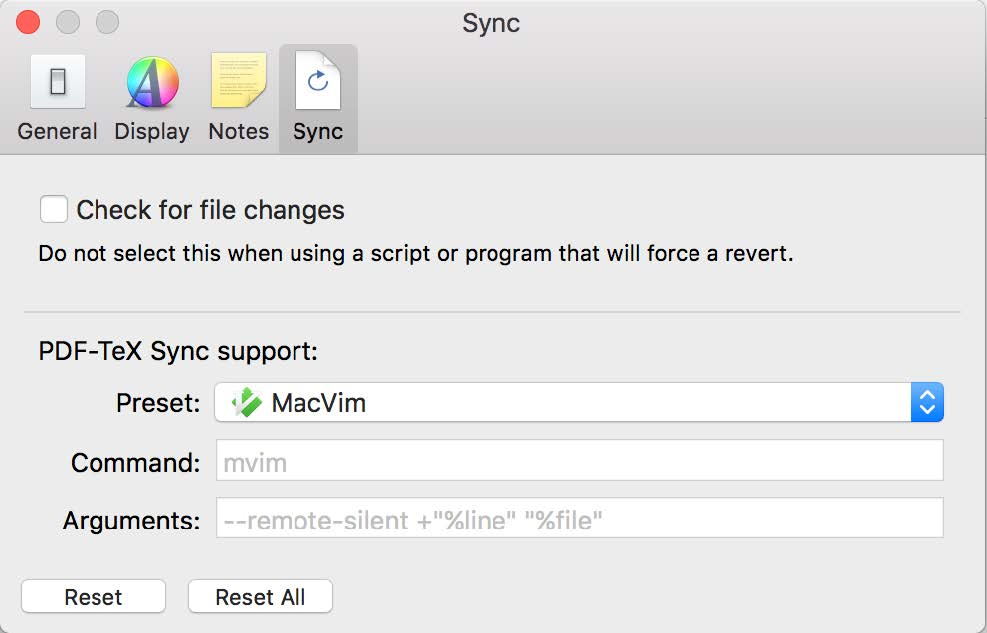
\includegraphics[width=0.6\linewidth]{pics/Skim-MacVim.jpg}
            \caption{Configure the Skim to select MacVim}
        \end{figure}

    \item (For both \textbf{Mac} and \textbf{Windows}) Install \TeX{}
        Studio, with default configuration, to folder where you
        prefer. 

        \textbf{Explanation}: \TeX{} Studio provides very useful list
        of commands, reference tables for editing \LaTeX.

    \item (For \textbf{Windows} only) Install \texttt{Python} with
        mostly default configuration. Note that you should add
        \texttt{Python} to the system \texttt{PATH} variable too:
        \begin{figure}[H]
            \centering
            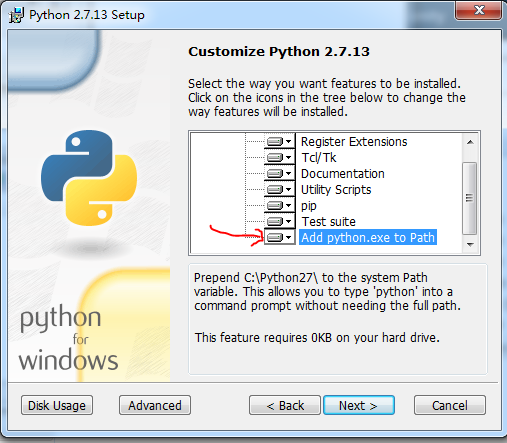
\includegraphics[width=0.6\linewidth]{pics/3.PNG}
        \end{figure}

    \item Install a handy but advanced (better than Notepad) text
        editor. One Windows, I prefer Notepad++ for its small file
        size. On Mac, I think Sublime Text is a better one.

    \item Set up Vim configuration, and some Vim plugins. Vundle is
        the first and most important Vim plugin that manages other
        plugins (a plugin that manages plugins). Installation is
        straight forward. 
        
        \begin{enumerate}
            \item Clone Vundle with git to somewhere you like:

                On Windows:

                \texttt{\footnotesize git clone
                https://github.com/VundleVim/Vundle.vim.git}

                Then move the downloaded folder to \path{Vim Installation
                Folder > vimfiles > bundle > Vundle.vim} (create new empty
                folder is required).

                On Mac, you could simply type this:

        \end{enumerate}
            
\begin{verbatim}
git clone https://github.com/VundleVim/Vundle.vim.git ~/.vim/bundle/ Vundle.vim
\end{verbatim}

        \begin{enumerate}
            \setcounter{enumii}{1}
            \item Get Vim configuration file.
                
                \textbf{For Windows}:
                
                Copy my configuration text to file \texttt{\_vimrc},
                which can be found in the folder \path{where Vim is
                installed}. My configuration text can be found here:
                \href{https://github.com/we-taper/vimConfig/blob/master/_vimrc}
                {My GitHub Link}.

                \textbf{For Mac}:

                Download the
                \href{https://raw.githubusercontent.com/we-taper/vimConfig/master/vimrc-mac}{Mac
                version} and copy it to \path{.\.vimrc}.

            \item Modify some part of my configuration to suit your
                computer setup:
                \begin{itemize}
                    \item Adjust your color scheme on this line:

                        \command{ colorscheme~Atelier\_SulphurpoolDark }

                    \item (For \textbf{Windows} only) Let Vim find
                        python properly. You will find a line starts
                        with \menu{let \$PYTHONPATH=}, followed by
                        some path, and you should change all of them
                        to the correct path to locate the python files
                        you installed.

                    \item Choice a proper font. Search for: \menu{if
                        has('gui\_running')} in my vimrc file, and
                        adjust it to meed your needs.
                \end{itemize}

            \item Restart Vim to make the new Vim configuration take
                effect. It turns out that on Mac, you just have to
                close Macvim, and it will restart automatically again,
                unless you right click and say quit from the task bar.

            \item Then do \menu{:PluginList} and then
                \menu{:PluginInstall} in Vim, and restart Macvim. 

        \end{enumerate}
        
\end{enumerate}

\section{Possible Problems}
\label{sec:Possible Problems}

If you ever did Chinese latex, you will need \texttt{xelatex} engine,
and to tell \texttt{latexmk} (used by \texttt{vimtex} to make latex into
pdf) use xelatex. Then you should create a file named
\menu{.latexmkrc} in the same directory as your latex file, and put the following content into
that file:
\begin{verbatim}
$pdflatex=q/xelatex -synctex=1 %O %S/
\end{verbatim}

\printnomenclature
\section{License}
The entire content of this work (including the source code
for TeX files and the generated PDF documents) by 
Hongxiang Chen (nicknamed we.taper, or just Taper) is
licensed under a 
\href{http://creativecommons.org/licenses/by-nc-sa/4.0/}{Creative 
Commons Attribution-NonCommercial-ShareAlike 4.0 International 
License}. Permissions beyond the scope of this 
license may be available at 
\href{http://www.google.com/recaptcha/mailhide/d?k=015LguzBJigi0rpyuJRqLoig==\&c=p1c-M-mm7ZcjUCkTuZZa9eEPHRVk6paN0694iazlQy8=}
{[My Email Address(Click)]}.
\end{document}
